\documentclass[11pt,a4paper]{article}

%==============================================================================%

\usepackage{a4wide}
\usepackage{amsmath,amssymb}
\usepackage[utf8]{inputenc}
\usepackage{float}
\usepackage{graphicx}
\usepackage{listings}
\usepackage{multicol}

%==============================================================================%

\newcommand{\assignmentnumber}{8}

\newcommand{\colbreak}{\vfill{\ }\columnbreak}

\newcommand{\half}{\frac{1}{2}}
\newcommand{\modulus}[1]{\left|#1\right|}
\newcommand{\conjugate}[1]{\bar{#1}}
\newcommand{\degree}{^{\circ}}
\newcommand{\limit}[2]{\lim_{#1 \rightarrow #2}}

\newcommand{\figref}[1]{fig. \ref{fig:#1}}
\newcommand{\eqnref}[1]{(\ref{eqn:#1})}

\newcommand{\fig}[4]
{
    \begin{figure}[H]
        \centering
        \includegraphics[scale=#3]{figures/#2}
        \caption{#4}
        \label{fig:#1}
    \end{figure}
}

\DeclareMathOperator{\re}{Re}
\DeclareMathOperator{\im}{Im}

\renewcommand\thesection{\assignmentnumber.\arabic{section}}
\renewcommand\thesubsection{\alph{subsection})}

%==============================================================================%

\title{MatIntro Pointopgave \assignmentnumber}
\author
{
    Casper B. Hansen\\
    University of Copenhagen\\
    {\tt fvx507@alumni.ku.dk}
}
\date{\today}

%==============================================================================%

\begin{document}

% \maketitle


% 8.1
\section
{
    \mdseries
    Benyt Maple til at finde alle stationære punkter for funktionen $f :
    \mathbb{R}^2 \rightarrow \mathbb{R}$ givet ved
}
\begin{align}
    f(x,y) = x(8x^2 + 5x + \cos y)
    \label{eqn:8.1-function}
\end{align}
\section*
{
    \mdseries
    og til at afgøre, om der er tale om lokalt maksimum, minimum eller
    sadelpunkt for hvert af dem. Tegn med Maple grafen for $f$ i nærheden af
    et sadelpunkt, til illustration af det punkts type.
}
\begin{multicols}{2}
I Maple løser jeg for de stationære punkter ved

\begin{lstlisting}
f := (x,y) -> x (8x^2 + 5x + cos(y))
fx := diff(f(x,y), x)
fy := diff(f(x,y), y)
ps := solve(fx=0, fy=0)
\end{lstlisting}

hvilket giver mig de stationære punkter
\begin{align*}
    p_1 = \left( 0, \half \pi \right) &\quad \\
    p_2 = \left( -\frac{1}{6}, 0 \right) &\quad
    p_3 = \left( -\frac{1}{4}, 0 \right) \quad \\
    p_4 = \left( -\half, \pi \right) &\quad
    p_5 = \left( \frac{1}{12}, \pi \right)
\end{align*}

\colbreak

\begin{figure}[H]
    \centering
    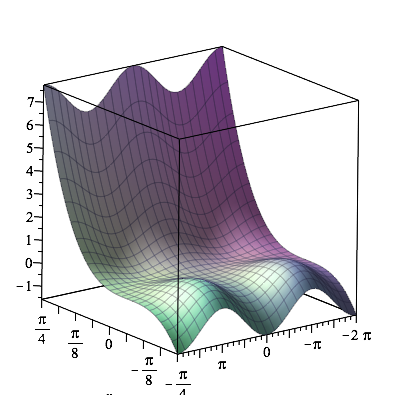
\includegraphics[scale=0.4]{figures/8-1-sadel.png}
    \caption{Grafen for $f$ i $x \in [-\frac{1}{4}\pi,\frac{1}{4}\pi]$ og
    $y \in [-2\pi,2\pi]$}
    \label{fig:8.1-sadel}
\end{figure}

\end{multicols}

Vi anvender nu ABC-kriteriet, og beregner $A$, $B$ hhv. $C$
\begin{align}
    A = \frac{\partial^2 f}{\partial x^2} = 48x + 10
    \qquad
    B = \frac{\partial^2 f}{\partial x \partial y} = -\sin y
    \qquad
    C = \frac{\partial^2 f}{\partial x^2} = -x \cos y
\end{align}
Med disse kan vi nu bestemme $D = AC - B^2$ for hvert af de stationære
punkter
\begin{align}
    D(p_1) = -1 \qquad
    D(p_2) = \frac{1}{3} \qquad
    D(p_3) = -\half \qquad
    D(p_4) = 7 \qquad
    D(p_5) = \frac{7}{6}
\end{align}

Vi har da, jvf. sætning 3.4 TK, at $p_1$ og $p_3$ er sadelpunkter, idet
$D < 0$, og de øvrige er lokale minima eller maxima. For at finde ud af, om
de er minima eller maxima beregner vi $A$ for dem
\begin{align}
    A(p_2) = 2 \qquad
    A(p_4) = -14 \qquad
    A(p_5) = 14
\end{align}

Igen, jvf. sætning 3.4 TK har vi, at $p_2$ og $p_5$ er lokale minima, idet
$A > 0$ og ligeledes $p_4$ er lokalt maximum, idet $A < 0$.

% 8.2
\section
{
    \mdseries (Uden Maple)\\
    Vi lader $D$ betegne den halve enhedscirkelskive
}
\begin{align}
    D = \{ (x,y) \in \mathbb{R}^2 | x^2 + y^2 \leq 1, x \geq 0 \}
\end{align}
\section*
{
    \mdseries
    og betragter funktionen $f : D \rightarrow \mathbb{R}^2$ givet ved
}
\begin{align}
    f(x,y) = 4xy^2 - x^2
\end{align}
\section*
{
    \mdseries
    Giv en begrundelse for, at $f$ har en størsteværdi og en mindsteværdi i
    $D$. Bestem disse værdier og angiv, i hvilke punkter af $D$ disse
    værdier antages.
}
\begin{multicols}{2}
    Mængden $D$ er lukket med $0 \leq x \leq 1$ og $-1 \leq y \leq 1$, og
    funktionen $f$ er kontinuert. Jvf. ekstremalværdisætningen 2.42 TK, må
    $f$ da også have største- hhv. mindsteværdi i $D$.

    Det er let at se ud fra ledene i $f$, at for at finde mindsteværdien,
    bør vi maksimere $x^2$ og minimere $4xy^2$, og omvendt for
    størsteværdien. Mindsteværdien er da $f(\pm 1,0) = -1$ og størsteværdien
    er da $f(1,\pm 1) = 3$. Dette fremgår også tydeligt af grafen til højre.
    
    \iffalse
    Lad os regne efter; vi bemærker at tværsnittet i $x$ hhv. $y$ er begge
    parabler

    \begin{align}
        \frac{\partial f}{\partial x} = 4y^2 - 2x
        \qquad
        \frac{\partial^2 f}{\partial x^2} = 4y^2 - 2 \\
        \frac{\partial f}{\partial y} = 8xy - x^2
        \qquad
        \frac{\partial^2 f}{\partial y^2} = 8x - x^2
    \end{align}
    \fi

    \colbreak

    \fig{8.2}{8-2-f.png}{0.5}{Graf for $f$ i $x \in [0,1]$ og $y \in [-1,1]$}

\end{multicols}


% 8.3
\newpage
\section
{
    \mdseries (Uden Maple) \\
    Ved forsendelse af såkaldte ruller, altså pakker i cylinderform, kræver
    postvæsenet i Langbortistan, at summen af længden $l$ og tre en halv
    gange diameteren $d$ højst må være 84cm. Hvad er den maksimale volumen
    af sådan en rulle?
    \\\\
    Redegør for, at opgaven kan løses ved at bestemme maksimum for en
    funktion $V(l,d)$ defineret i en afsluttet og begrænset delmængde af
    $\mathbb{R}^2$ (optimering under bibetingelser). Løs dette
    optimeringsproblem dels ved elimination af én af de variable og dels ved
    brug af Lagranges metode.
}
\begin{multicols}{2}
    Betingelsen der opstilles af postvæsenet i Langbortistan er givet ved
    \begin{align}
        l + \frac{7}{2}d \leq 84\text{cm}
    \end{align}
    og funktionen $V(l,d)$ for volumen er givet ved
    \begin{align}
        V(l,d) = \pi l r^2 = \frac{\pi l d^2}{4}\text{, }r=\frac{d}{2}
    \end{align}

    Vi skal altså finde størsteværdien af $V(l,d)$ på mængden
    \begin{align}
        \{ (l,d) \in \mathbb{R}^2{\ }|{\ } l + \frac{7}{2}d = 84 \}
    \end{align}

    Isolerer vi $l$ hhv. $d$ har vi, at
    \begin{align}
        l = 84 - \frac{7}{2}d
        \qquad
        d = 24 - \frac{2l}{7}
    \end{align}

    Vi kan da udtrykke $V$ som en funktion af én variabel --- $l$ eller $d$.
    Her givet på polynomiumform, da det gør differentiation lettere.
    \begin{align}
        V(l) = \frac{\pi}{49} l^3 - \frac{24 \pi}{7} l^2 + 144 \pi l \\
        V(d) = 21 \pi d^2 - \frac{7 \pi}{8} d^3
    \end{align}

    Lad os differentiere disse
    \begin{align}
        V(l) = \frac{3 \pi}{49} l^2 - \frac{48 \pi}{7} l + 144 \pi \\
        V(d) = 42 \pi d - \frac{21 \pi}{8} d^2
    \end{align}

    Da $V(d)$ er et andengradspolynomium vælger vi at løse for $V'(d) = 0$
    \begin{align}
        &=\frac{-(42\pi) \pm \sqrt{(42\pi)^2 - 4 (-21\pi/8) \cdot 0}}{2 (-21\pi/8)} \\
        &= \frac{-42\pi \pm 42\pi}{-42\pi(1/8)} = (1 \pm 1)8 = 16\\
    \end{align}

    Idet vi ikke kan have en negativ diameter, må $d = 16$

    Da vi nu kender $d$ indsætter vi og beregner $l$
    \begin{align}
        l &= 84 - \frac{7}{2} \cdot 16
           = 84 - \frac{112}{2}
           = 28
    \end{align}

    Den maksimale volumen af pakken må da være
    \begin{align}
        V(28,16) &= \frac{\pi 28 \cdot 16^2}{4}
                  = \pi 7 \cdot 16^2
                  = 1792\text{cm}^3
    \end{align}

    \colbreak

    Lad os nu løse samme problemstilling vha. Lagranges multiplikationsmetode.
    
    Vi beregner gradienterne for betingelsen, som vi vil benævne ved $g$, og
    volumen
    \begin{align}
        \nabla g(l,d) = (1, \frac{7}{2})
        \quad
        \nabla V(l,d) = (\frac{\pi d^2}{4}, \frac{2\pi l d}{4})
    \end{align}
    
    Vi skal nu løse ligningssættet, som opfylder
    \begin{align}
        1 = \lambda \frac{\pi d^2}{4}
        \quad
        \frac{7}{2} = \lambda \frac{2 \pi l d}{4}
        \quad
        84 = \frac{\pi l d^2}{4}
        \\
        4 = \lambda \pi d^2
        \quad
        7 = \lambda \pi l d
        \quad
        336 = \pi l d^2
    \end{align}

    Øv. Noget gik galt, og kan ikke nå at rette det :(

\end{multicols}

\end{document}
